\documentclass[11pt,a4paper]{article}
\usepackage[utf8]{inputenc}
\usepackage[T1]{fontenc}
\IfFileExists{lmodern.sty}{\usepackage{lmodern}}{}
\usepackage{amsmath,amssymb,amsthm,bm}
\usepackage{booktabs}
\usepackage{graphicx}
\usepackage[margin=2.5cm]{geometry}
\usepackage{hyperref}
\usepackage{listings}
\usepackage{xcolor}

\lstset{basicstyle=\ttfamily\small,columns=fullflexible,frame=single,
        backgroundcolor=\color{gray!6},breaklines=true,
        literate={Γ}{{$\Gamma$}}1 {θ}{{$\theta$}}1 {Θ}{{$\Theta$}}1 {π}{{$\pi$}}1 {ρ}{{$\rho$}}1}

\newtheorem{proposition}{Proposition}
\newcommand{\avg}[1]{\{\!\{#1\}\!\}}
\newcommand{\jump}[1]{[\![#1]\!]}
\newcommand{\qh}{\hat{\bm q}}
\newcommand{\q}{\bm q}
\newcommand{\thb}{\bar\theta}
\newcommand{\pib}{\bar\pi}

\title{The fast linear operator of the Euler equations in\\
potential-temperature form: hybridized DG with LMARS flux,\\
relaxed trace conditions and time integration without elimination}
\author{Documentation of \texttt{hdg\_relax\_theta.py} / \texttt{HDGRelaxTheta.jl}}
\date{\today}

\begin{document}
\maketitle

\begin{abstract}
We derive and discretize the linear fast operator of the one-dimensional (vertical)
compressible Euler equations in the variables $(\rho,\rho w,\rho\theta)$, as needed for
the fast (acoustic) part of a split-explicit method. Momentum advection is removed, $\theta$ is
frozen in the $\rho\theta$ equation, and the pressure is written as
$p=\frac{p}{\rho\theta}\,\rho\theta$ with $\frac{p}{\rho\theta}$ frozen. The resulting system is
linear in the full state. It is discretized by a hybridized DG (HDG) method whose stabilization
$\bm T=|\bm A|$ reproduces the LMARS flux exactly. The trace conditions are relaxed into evolution
equations, and the coupled element/trace system is integrated without static condensation,
either monolithically (SDIRK4) or with an IMEX scheme whose implicit stage is local per face.
Frozen coefficients are continuous piecewise polynomials, which makes discrete hydrostatic
states exactly steady. The operator accepts a constant slow tendency, so it can be used as the
fast part of a split-explicit scheme.
\end{abstract}

\tableofcontents

%=====================================================================
\section{Model and linearization}
%=====================================================================
\subsection{Full equations}
In a vertical column with $m=\rho w$ and $\Theta=\rho\theta$,
\begin{align}
\partial_t\rho + \partial_z m &= 0,\\
\partial_t m + \partial_z(m w + p) &= -\rho g,\\
\partial_t\Theta + \partial_z(\theta m) &= 0,\qquad
p = p_{00}\Big(\frac{R\,\Theta}{p_{00}}\Big)^{\gamma}.
\end{align}

\subsection{Linearization (fast operator)}
Let a frozen state (bars) be given, for example the current slow state or a reference profile.
The linearization consists of three steps.
\begin{enumerate}
\item Remove momentum advection: $\partial_z(mw)\to0$.
\item Freeze $\theta$ in the $\Theta$ equation: $\partial_z(\theta m)\to\partial_z(\thb\,m)$.
\item Write $p=\dfrac{p}{\Theta}\,\Theta$ and freeze the ratio:
      $p\to\pib\,\Theta$, with $\pib=\bar p/\bar\Theta = R\,\bar\Pi$ ($\Pi$ = Exner function).
\end{enumerate}
This gives
\begin{equation}\label{eq:fast}
\boxed{\;
\partial_t\rho+\partial_z m=0,\qquad
\partial_t m+\partial_z(a\,\Theta+b)=-g\rho,\qquad
\partial_t\Theta+\partial_z(\thb\,m)=0,\;}
\end{equation}
with $a=\pib$ and $b=0$. The system is linear in the \emph{full} state $\q=(\rho,m,\Theta)$,
not in perturbations. In flux form,
$\partial_t\q+\partial_z(\bm A\q+b\,\bm e_m)=\bm S\q$ with
\begin{equation}
\bm A(z)=\begin{pmatrix}0&1&0\\0&0&a\\0&\thb&0\end{pmatrix},\qquad
\bm S=\begin{pmatrix}0&0&0\\-g&0&0\\0&0&0\end{pmatrix}.
\end{equation}

\subsection{Sound speed and the factor \texttt{pfac}}
The eigenvalues of $\bm A$ are $0,\pm c$ with
\begin{equation}
c^2 = a\,\thb = \frac{\bar p}{\bar\Theta}\,\frac{\bar\Theta}{\bar\rho}=\frac{\bar p}{\bar\rho}=R\bar T .
\end{equation}
Freezing $p/\Theta$ therefore gives the isothermal (Newtonian) sound speed, smaller than the
adiabatic one, $\gamma R\bar T$, by a factor $\sqrt\gamma$ (287 versus 340\,m/s at 288\,K).
The tangent linearization would use $\partial p/\partial\Theta=\gamma p/\Theta$. In a
split-explicit scheme the slow tendency can carry the remainder $p-\pib\Theta$, so the
choice is a design decision. The code provides
\begin{equation}
p_{\rm lin}= a\,\Theta + b,\qquad a=\texttt{pfac}\,\pib,\qquad b=(1-\texttt{pfac})\,\bar p,
\end{equation}
where $\texttt{pfac}=1$ (default) is the linearization above and $\texttt{pfac}=\gamma$ is the
tangent-linear pressure with $c^2=\gamma R\bar T$. The constant $b$ keeps $p_{\rm lin}(\bar\Theta)=\bar p$,
so the frozen hydrostatic state remains steady for any \texttt{pfac}.

\subsection{Use in a split-explicit method}
With the full nonlinear operator $\mathcal N$ and the fast operator $\mathcal L$ of
\eqref{eq:fast}, frozen at the slow level $\q^n$, the fast system integrated over the small steps is
\begin{equation}
\partial_t\q = \mathcal L(\q) + \bm F_{\rm slow},\qquad
\bm F_{\rm slow}=\mathcal N(\q^n)-\mathcal L(\q^n)\ \ (\text{or a multistage variant}),
\end{equation}
with $\bm F_{\rm slow}$ constant over the small steps (e.g.\ \cite{wicker2002}). Every run accepts
\texttt{F\_slow} as a constant tendency. The function \texttt{tendency(q)} returns $\mathcal L(\q)$
in the HDG limit, so $\bm F_{\rm slow}$ can be formed directly.

%=====================================================================
\section{HDG discretization with LMARS flux}
%=====================================================================
\subsection{Local problem}
On $K_e=[z_{e-1/2},z_{e+1/2}]$ the element unknowns lie in $P_p(K_e)^3$ (Legendre basis), and each
face carries a single-valued trace $\qh_f\in\mathbb R^3$. For all $\bm v\in P_p(K)^3$,
\begin{equation}\label{eq:local}
(\bm v,\partial_t\q_h)_K = (\partial_z\bm v,\bm A\q_h+b\,\bm e_m)_K + (\bm v,\bm S\q_h)_K
 - \sum_{f\in\partial K}\bm v(z_f)^{\mathsf T}\widehat{\bm F}_{K,f},
\end{equation}
\begin{equation}\label{eq:hdgflux}
\widehat{\bm F}_{K,f}=\big(\bm A_f\qh_f+b_f\bm e_m\big)\,n+\bm T_f\big(\q_h|_K(z_f)-\qh_f\big).
\end{equation}

\subsection{Stabilization and the LMARS flux}
Since the eigenvalues of $\bm A$ are $0,\pm c$, we have $|\bm A|=\bm A^2/c$, i.e.
\begin{equation}
\bm T_f=|\bm A_f|=\begin{pmatrix}0&0&a_f/c_f\\0&c_f&0\\0&0&c_f\end{pmatrix},\qquad c_f^2=a_f\thb_f .
\end{equation}
\paragraph{Trace conditions.}
\begin{itemize}
\item Interior faces: conservativity
  $\bm T_f(\q_L-\qh_f)+\bm T_f(\q_R-\qh_f)=\bm 0$. The $m$ and $\Theta$ rows give
  $\hat m=\avg m$ and $\hat\Theta=\avg\Theta$. $\hat\rho$ enters no flux, because the first
  columns of $\bm A$ and $\bm T$ vanish, and is set to $\avg\rho$. So $\qh=\avg{\q}$.
\item Walls: $\qh_f=\operatorname{diag}(1,0,1)\,\q_{\rm int}$, i.e.\ $\hat m=0$.
\end{itemize}
Inserting $\qh=\avg{\q}$ into \eqref{eq:hdgflux} with $\jump{\cdot}=(\cdot)_R-(\cdot)_L$ gives
\begin{equation}\label{eq:lmars}
\widehat{\bm F}=\begin{pmatrix}m^\ast\\ p^\ast\\ \thb_f\,m^\ast\end{pmatrix},\qquad
m^\ast=\avg m-\frac{a_f\jump{\Theta}}{2c_f}=\avg m-\frac{\jump{p_{\rm lin}}}{2c_f},\qquad
p^\ast=a_f\avg\Theta+b_f-\frac{c_f}{2}\jump m .
\end{equation}
This is the LMARS flux~\cite{chen2013} for \eqref{eq:fast}: interface momentum and pressure from
the acoustic Riemann invariants, and the $\Theta$ flux $\thb\,m^\ast$, in which upwinding of
$\theta$ is irrelevant because $\theta$ is frozen. The code checks this identity to round-off.

\subsection{Frozen coefficients}
The coefficients $a$, $\thb$, $b$ are represented as \emph{continuous} piecewise polynomials of
degree $p$, interpolated at Gauss--Lobatto nodes. This matches the situation in a DG model, where
they come from the slow state (one would take a continuous reconstruction there as well).
All volume integrands are then polynomials of degree at most $3p$. The code uses $2p+2$ Gauss
points, which integrate them exactly, and face values are single-valued.

\subsection{Matrix form and relaxation}
With all element coefficients in $\q$ and traces in $\qh$,
\begin{equation}\label{eq:relax}
\begin{pmatrix}\bm M&\bm 0\\\bm 0&\varepsilon\bm I\end{pmatrix}
\frac{d}{dt}\begin{pmatrix}\q\\\qh\end{pmatrix}
=\begin{pmatrix}\bm K&\bm G\\\bm H&-\bm I\end{pmatrix}
\begin{pmatrix}\q\\\qh\end{pmatrix}
+\begin{pmatrix}\bm f_b+\bm M\bm F_{\rm slow}\\\bm 0\end{pmatrix}.
\end{equation}
Here $\bm f_b$ collects the affine pressure part $b$, and $\bm H$ is the face-local trace
condition ($\qh=\bm H\q$). For $\varepsilon=0$ this is the HDG/LMARS scheme as an index-1 DAE.
For $\varepsilon>0$ the trace condition is relaxed. In both cases the element unknowns are
\emph{not} eliminated. The relaxation error is $\mathcal O(\varepsilon c/h)$, because the trace
defect $\qh-\bm H\q\approx-\varepsilon\bm H\dot\q$ enters through $\bm M^{-1}\bm G\sim c/h$.

%=====================================================================
\section{Time integration}
%=====================================================================
\begin{itemize}
\item \texttt{method="dirk"}: five-stage, fourth-order, L-stable and stiffly accurate SDIRK
of Hairer--Wanner~\cite{hairer} ($a_{ii}=1/4$). Each stage solves
$(\mathcal M-\tfrac{\Delta t}{4}\bm L)\bm Y_i=\mathcal M\bm U^n+\Delta t\sum_{j<i}a_{ij}(\bm L\bm Y_j+\bm f)+\tfrac{\Delta t}{4}\bm f$
with one sparse LU of the full coupled matrix. It is valid for every $\varepsilon\ge0$.
\item \texttt{method="imex"}: ARS(2,2,2)~\cite{ars}, with the element part explicit and the
relaxation implicit. The implicit stage is
$\qh^{(i)}=(\qh^\ast+k\bm H\q^{(i)})/(1+k)$ with $k=\Delta t\,a^I_{ii}/\varepsilon$. It is local per
face, so there is no linear solve. It is asymptotic preserving: for $\varepsilon\to0$ it becomes an
explicit DG/LMARS scheme under the CFL condition $\Delta t\lesssim h/(c(2p+1))$.
\end{itemize}
The explicit variant is the natural fast integrator of a split-explicit method. The monolithic
variant gives a vertically implicit (HEVI-type) option.

%=====================================================================
\section{Properties}
%=====================================================================
\begin{proposition}[Discrete hydrostatic balance]\label{prop:wb}
Let $\Theta_h$ be continuous and piecewise $P_p$, $m_h=0$, and
$\rho_h=-\Pi_p\,\partial_z(a\Theta_h+b)/g$ element-wise ($\Pi_p$ = $L^2$ projection), with
$\qh=\bm H\q_h$. Then $(\q_h,\qh)$ is a steady state of \eqref{eq:relax} with $\bm F_{\rm slow}=0$,
for every $\varepsilon\ge0$ and every \texttt{pfac}.
\end{proposition}
\begin{proof}
$\Theta_h$ is continuous and $m_h=0$, so $\hat\Theta_f=\Theta_h(z_f)$, $\hat m_f=0$ and
$\bm H\q-\qh=0$. In \eqref{eq:hdgflux}, the $\rho$ row $\hat m\,n+\tfrac{a}{c}(\Theta_h-\hat\Theta)$
and the $\Theta$ row $\thb\hat m\,n+c(\Theta_h-\hat\Theta)$ vanish, and so do their volume terms.
The $m$ row of the flux is $p_{\rm lin}(z_f)\,n$, with $p_{\rm lin}=a_h\Theta_h+b_h$ continuous.
Since the quadrature is exact,
$(\partial_zv,p_{\rm lin})_K-[v\,p_{\rm lin}]_{\partial K}-g(v,\rho_h)_K
=-(v,\partial_zp_{\rm lin}+g\rho_h)_K=0$ for all $v\in P_p$, by the definition of $\rho_h$.
\end{proof}
The code builds such states with \texttt{balanced\_state} (Julia) or \texttt{hydrostatic\_rho}
(Python). An analytic background that is merely projected is steady only up to truncation error,
$\mathcal O(h^{p})$ in $\partial_t\q$ (Table~\ref{tab:wb}).

\paragraph{Conservation.} Summing the two one-sided fluxes at a face gives
$\bm T_f(\q_L+\q_R-2\qh)=2\bm T_f\,\varepsilon\dot{\qh}$. Mass, momentum and $\Theta$ are therefore
conserved to round-off for $\varepsilon=0$, and up to $\mathcal O(\varepsilon)$ otherwise.

%=====================================================================
\section{Verification}
%=====================================================================
All numbers come from the Python implementation (\texttt{run\_tests\_theta.py}). The Julia port
implements the same algorithm and prints the same tests, with these values in its comments.

\subsection{Convergence}
Constant frozen coefficients $\pib=R$, $\thb=300$\,K ($c=293$\,m/s), periodic domain of 2000\,m,
exact normal mode of \eqref{eq:fast} (pressure amplitude 100\,Pa), one acoustic transit.
\begin{table}[h]\centering
\caption{$L^2$ error in $\Theta$; the rates for $\rho$, $m$, $\Theta$ coincide.}\label{tab:conv}
\begin{tabular}{llccccc}\toprule
method & $p$ & $N_e=8$ & 16 & 32 & 64 & rate\\\midrule
DIRK, $\varepsilon=0$ & 1 & 6.44e-1 & 1.30e-1 & 3.00e-2 & 7.31e-3 & 2.04\\
 & 2 & 2.93e-2 & 3.65e-3 & 4.56e-4 & 5.70e-5 & 3.00\\
 & 3 & 1.39e-3 & 8.81e-5 & 5.51e-6 & 3.44e-7 & 4.00\\
DIRK, $\varepsilon=10^{-9}h/c$ & 3 & 1.39e-3 & 8.81e-5 & 5.51e-6 & 3.79e-7 & 3.86\\
IMEX, $\varepsilon=10^{-9}h/c$ & 1 & 6.48e-1 & 1.31e-1 & 3.00e-2 & 7.33e-3 & 2.04\\
 & 2 & 3.20e-2 & 4.85e-3 & 9.19e-4 & 2.07e-4 & 2.15\\\bottomrule
\end{tabular}
\end{table}

\begin{table}[h]\centering
\caption{$L^2$ error in $\Theta$ versus $\varepsilon c/h$ ($N_e=16$, $p=3$); the $\varepsilon=0$
reference is $8.81\cdot10^{-5}$ (DIRK) and $1.63\cdot10^{-3}$ (IMEX, time-error dominated).}\label{tab:eps}
\begin{tabular}{lccccccc}\toprule
$\varepsilon c/h$ & $10^{-8}$ & $10^{-7}$ & $10^{-6}$ & $10^{-5}$ & $10^{-4}$ & $10^{-3}$ & $10^{-2}$\\\midrule
DIRK & 8.81e-5 & 8.95e-5 & 1.79e-4 & 1.56e-3 & 1.55e-2 & 1.55e-1 & 1.52e+0\\
IMEX & 1.63e-3 & 1.62e-3 & 1.48e-3 & 1.31e-4 & 1.39e-2 & 1.53e-1 & 1.52e+0\\\bottomrule
\end{tabular}
\end{table}

\subsection{Hydrostatic balance}
Lapse-rate atmosphere ($T_0=288$\,K, $\Gamma=6.5$\,K/km), walls, $[0,10]$\,km, $N_e=40$, $p=3$,
discrete hydrostatic state from Proposition~\ref{prop:wb} with $\Theta_h$ = interpolant of $\bar\Theta$.
\begin{table}[h]\centering
\caption{Maximum relative deviation after 200 steps, and residual of a projected background.}\label{tab:wb}
\begin{tabular}{lccc}\toprule
 & DIRK, $\varepsilon=0$ & DIRK, $\varepsilon=10^{-3}$ & IMEX, $\varepsilon=10^{-3}$\\\midrule
\texttt{pfac}$=1$ & 3.2e-13 & 4.3e-13 & 5.4e-15\\
\texttt{pfac}$=\gamma$ & 7.2e-13 & 8.0e-13 & 3.8e-15\\\midrule
\multicolumn{4}{p{0.85\textwidth}}{projected analytic background, $p=3$, $N_e=10,20,40,80$:
$\max|\dot\q|$ = 3.1e-6, 3.8e-7, 4.8e-8, 6.1e-9 (rate 3)}\\\bottomrule
\end{tabular}
\end{table}

\subsection{Slow forcing}
For a random state $\q^\ast$ (background plus noise) and $\bm F_{\rm slow}=-\mathcal L(\q^\ast)$,
the state stays at $\q^\ast$: $\max|\q-\q^\ast|=2.8\cdot10^{-12}$ (DIRK) and $2\cdot10^{-17}$
(IMEX) after 50 steps.

\subsection{Acoustic pulse between walls}
Discrete hydrostatic background plus a 100\,Pa pressure pulse ($\Theta'=p'/a$) at 3\,km,
$N_e=80$, $p=3$, $t=25$\,s.
\begin{table}[h]\centering
\caption{Sound speed at $z=0$, mass and $\Theta$ drift, trace residual.}\label{tab:wall}
\begin{tabular}{lcccc}\toprule
case & $c(0)$ [m/s] & $|\Delta$mass$|$ & $|\Delta\Theta|$ & trace res.\\\midrule
\texttt{pfac}$=1$, $\varepsilon=0$, DIRK & 287.5 & 2.2e-11 & 2.2e-8 & 6.7e-10\\
\texttt{pfac}$=1$, $\varepsilon=10^{-4}h/c$, IMEX & 287.5 & 1.4e-5 & 2.1e-3 & 1.5e-5\\
\texttt{pfac}$=\gamma$, $\varepsilon=0$, DIRK & 340.2 & 2.2e-11 & 5.6e-9 & 3.3e-10\\\bottomrule
\end{tabular}
\end{table}
The totals are of order $10^4$\,kg\,m$^{-2}$ (mass) and $3\cdot10^6$ ($\Theta$), so the
$\varepsilon=0$ drifts are at round-off level.

\IfFileExists{theta_convergence.png}{%
\begin{figure}[h]\centering
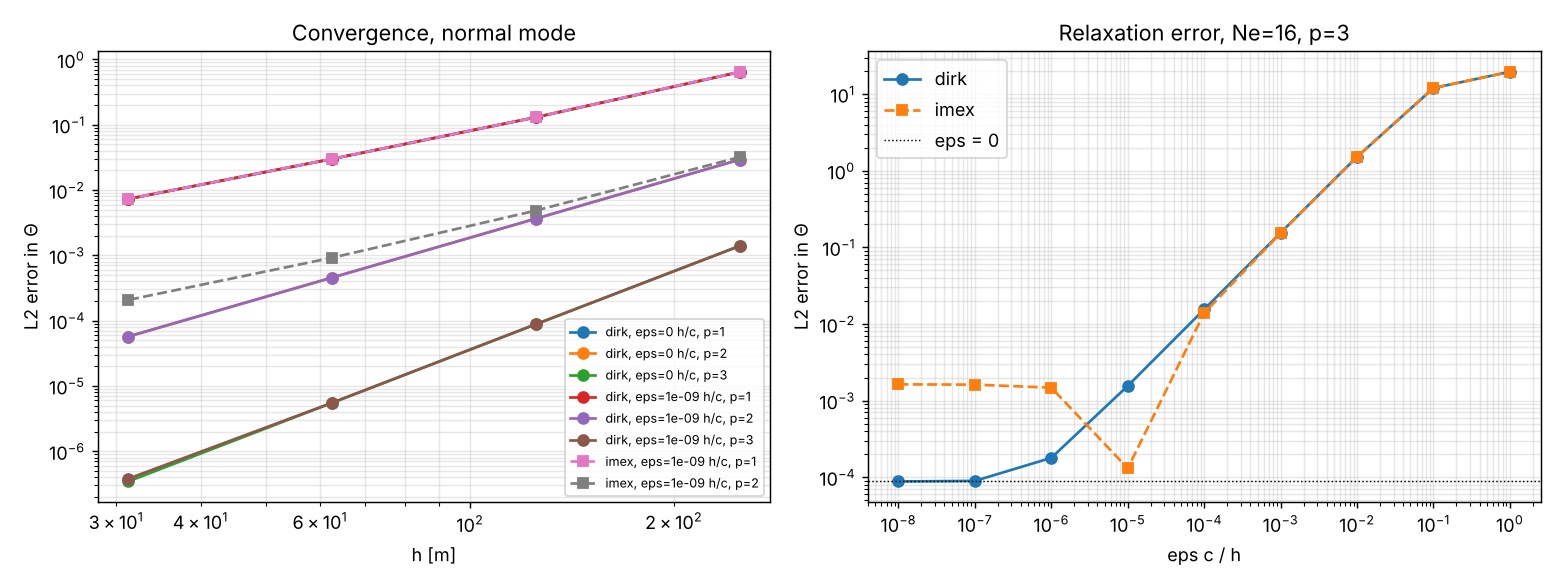
\includegraphics[width=\textwidth]{theta_convergence.png}
\caption{Left: convergence. Right: relaxation error versus $\varepsilon c/h$.}
\end{figure}}{}
\IfFileExists{theta_wall_demo.png}{%
\begin{figure}[h]\centering
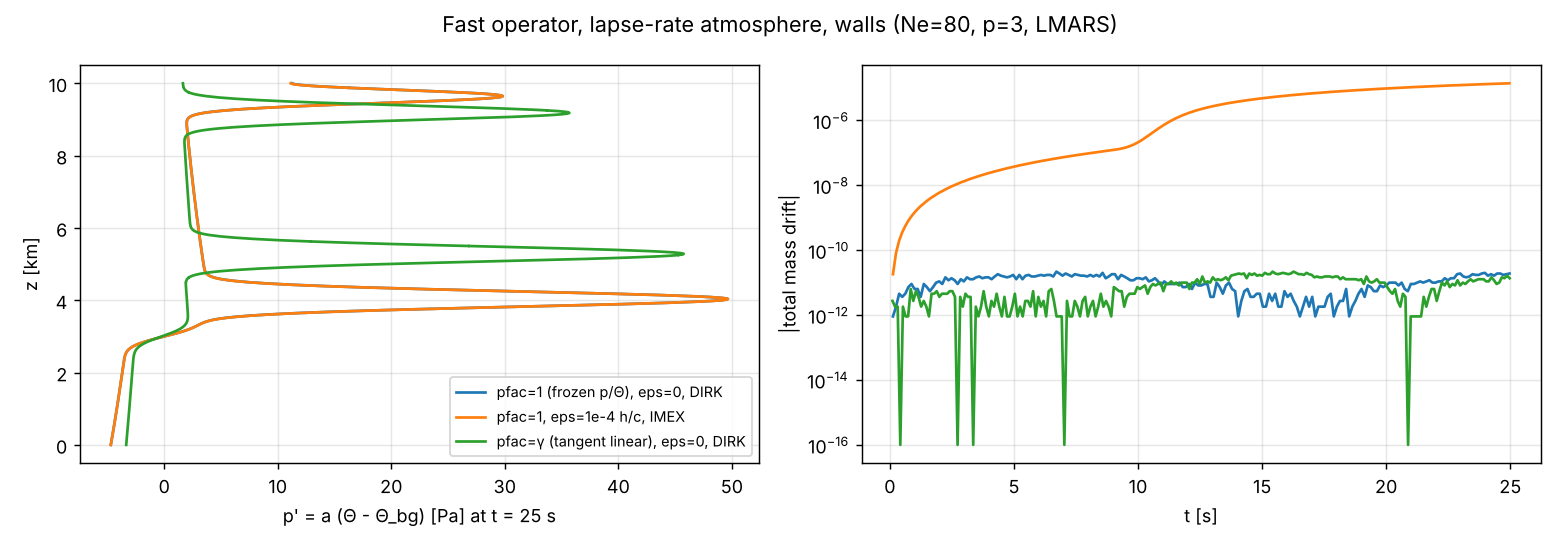
\includegraphics[width=\textwidth]{theta_wall_demo.png}
\caption{Pressure perturbation $a(\Theta-\Theta_{\rm bg})$ at $t=25$\,s for \texttt{pfac}$=1$ and
$\gamma$ (different wave speeds), and mass drift.}
\end{figure}}{}

%=====================================================================
\section{Code}
%=====================================================================
\begin{tabular}{ll}
\texttt{hdg\_relax\_theta.py} & Python solver (NumPy/SciPy)\\
\texttt{run\_tests\_theta.py} & Python tests and plots\\
\texttt{julia/HDGRelaxTheta.jl} & Julia module (standard library only)\\
\texttt{julia/run\_tests\_theta.jl} & Julia tests, writes CSV files\\
\end{tabular}

\subsection*{Usage (Julia)}
\begin{lstlisting}
include("HDGRelaxTheta.jl"); using .HDGRelaxTheta
atm = Atmosphere(T0 = 288.0, Γ = 0.0065)
fr  = frozen_from_atmosphere(atm; pfac = 1.0)      # or FrozenState(pi_fun, theta_fun; ...)
s   = HDGRelaxTh(80, 3, 0.0, 1.0e4, fr; bc = :wall, eps = 0.0)
q   = balanced_state(s, z -> atm_Theta(atm, z))     # discrete hydrostatic state
F   = zeros(s.nq)                                   # slow tendency (split-explicit)
U   = run!(s, initial_state(s, q), 0.05, 100; method = :imex, F_slow = F)
z, Q = evaluate(s, U[1:s.nq])                       # Q[1,:]=ρ, Q[2,:]=ρw, Q[3,:]=ρθ
\end{lstlisting}
Python:
\begin{lstlisting}
s = HDGRelaxTheta(Ne, p, zmin, zmax, FrozenState.from_atmosphere(atm, pfac),
                  bc="wall", eps=0.0)
U = s.run(U0, dt, n, method="imex", F_slow=F)
\end{lstlisting}
For frozen coefficients from a DG slow state, pass functions that evaluate a continuous
reconstruction of $\bar p/\bar\Theta$ and $\bar\theta$.

\begin{thebibliography}{9}
\bibitem{chen2013} X.~Chen, N.~Andronova, B.~van Leer, J.~E.~Penner, J.~P.~Boyd, C.~Jablonowski,
S.-J.~Lin, A control-volume model of the compressible Euler equations with a vertical Lagrangian
coordinate, \emph{Mon.\ Wea.\ Rev.} 141 (2013) 2526--2544.
\bibitem{cockburn2009} B.~Cockburn, J.~Gopalakrishnan, R.~Lazarov, Unified hybridization of
discontinuous Galerkin, mixed, and continuous Galerkin methods for second order elliptic
problems, \emph{SIAM J.\ Numer.\ Anal.} 47 (2009) 1319--1365.
\bibitem{ars} U.~M.~Ascher, S.~J.~Ruuth, R.~J.~Spiteri, Implicit-explicit Runge--Kutta methods for
time-dependent partial differential equations, \emph{Appl.\ Numer.\ Math.} 25 (1997) 151--167.
\bibitem{hairer} E.~Hairer, G.~Wanner, \emph{Solving Ordinary Differential Equations II: Stiff and
Differential-Algebraic Problems}, 2nd ed., Springer, 1996.
\bibitem{wicker2002} L.~J.~Wicker, W.~C.~Skamarock, Time-splitting methods for elastic models using
forward time schemes, \emph{Mon.\ Wea.\ Rev.} 130 (2002) 2088--2097.
\end{thebibliography}
\end{document}
